\documentclass[12pt]{article}

%%%% Load Packages %%%%
\usepackage[utf8]{inputenc}
\usepackage[english]{babel}
\usepackage{color}
\usepackage{xurl}
\usepackage{hyperref}
\usepackage[citestyle=authoryear, bibstyle=authoryear, sorting=nyt]{biblatex}
\usepackage{caption}
\usepackage{etoolbox}
\usepackage{fancyhdr}
\usepackage[margin=1in]{geometry}
\usepackage{graphicx}
\usepackage{parskip}
\usepackage{setspace}
\usepackage{titlesec}
\usepackage{booktabs}
\usepackage{multirow}
\usepackage{amsmath}
\usepackage[autostyle, english = american]{csquotes}
\usepackage{float} % for [H] placement specifier
\MakeOuterQuote{"}
\AtEveryBibitem{\ifentrytype{book}{\clearfield{isbn}}{}}
\addbibresource{ps_honors_thesis.bib}
\usepackage[acronym, nomain, nopostdot]{glossaries}
\makeglossaries

\titleformat{\section}{\fontsize{12}{14}\bfseries\centering}{\thesection}{0.5em}{}

%%%% List of Acronyms and abbreviations %%%%

\newacronym{acs}{ACS}{American Community Survey}
\newacronym{udp}{UDP}{Urban Displacement Project}
\newacronym{luof}{LUOF}{Lethal Use of Force}
\newacronym{ice}{ICE}{Index of Concentration at the Extremes}
\newacronym{poc}{PoC}{People of Color}

%%%% Head height %%%%
\setlength{\headheight}{15pt}
%%%% Line spacing %%%%
\setstretch{2}
%%%% Paragraph spacing %%%%
\setlength{\parskip}{0pt}
%%%% Define indentation length %%%%
\newlength{\myindent}
\setlength{\myindent}{0.5in}
%%%% Set the hanging indent %%%%
\setlength{\bibhang}{\myindent}
%%%% Redefine the citation command to use a colon instead of a comma and pp. %%%%
\DeclareFieldFormat{postnote}{#1}
\DeclareFieldFormat{multipostnote}{#1}
%%%% Use colon (APSA Style) in-text citations (author year, page) %%%%
\renewcommand*{\postnotedelim}{\addcomma\space}
%%%% Set global text alignment to ragged-right %%%%
%\raggedright
%%%% Paragraph indentation %%%%
\setlength{\parindent}{\myindent}

%%%% Font %%%%
% \setmainfont{Times New Roman}

%%%% Define a variable for the title %%%%
%\newcommand{\myTitle}{CONSTRUCTION UNION\dots{HISTORICAL-COMPARATIVE}}
\newcommand{\imageWidth}{0.8\textwidth}

%%%% Page style %%%%
\pagestyle{fancy}
\fancyhf{} % clear all header and footer fields
%\fancyhead[R]{\thepage} % page number on the right side
\fancyhead[R]{\hyperlink{toc}{\thepage}} % page number on the right side, linked to the TOC
%\fancyhead[L]{\small \myTitle}
\renewcommand{\headrulewidth}{1pt} % header rule

% Customize abstract page
\renewenvironment{abstract}
  {\par\noindent\centering\textbf{Abstract}\par}
  {\noindent\raggedright}
%  {\par}

% Redefine the quote environment
\renewenvironment{quote}
  {\list{}{\leftmargin=\parindent\rightmargin=0pt}%
   \item\relax}
  {\endlist}
  
% Redefine the quote environment to make it single-spaced 
% and remove vertical space before and add one at the end
\AtBeginEnvironment{quote}{\singlespacing\setlength{\topsep}{0pt}\setlength{\partopsep}{0pt}}
\AtEndEnvironment{quote}{\vspace{0.5\baselineskip}}

\begin{document}
\setstretch{1.25}
\begin{titlepage}
  \thispagestyle{fancy}
  \pagenumbering{gobble}
%  \fancyhead[L]{Running head: \myTitle}
  \renewcommand{\headrulewidth}{0pt} % header rule
  \centering
  \vspace*{2in}
  The Policing of the ``Reserve Army'':\par
  Economic Inequality and Police Killings\par
  \vspace{1.2in}
  {Matthew A. Carson\par}
  \vspace{12pt}
  Department of Political Science\par
  University of California, Los Angeles\par
  \vspace{0.5in}
  {March 22, 2024\par}
%  \vfill
%  \wordcount
\end{titlepage}

% Blank page so that the abstract does not begin on the back of the cover page.
\thispagestyle{empty} % Remove header and footer

\vspace*{\fill}
\hspace*{\fill}
\begin{center}
    \noindent{}\textit{This page intentionally left blank}
\end{center}
\hspace*{\fill}
\vspace*{\fill}

\clearpage

% Set page numbering to Roman for preliminary pages
\pagenumbering{roman}
\setstretch{2}
%\titlespacing*{\abstract}{0pt}{0pt}{0pt}
% Add abstract page
\begin{abstract}
This study examines the relationship between race, class, gentrification, and police use of lethal force (LUOF) in U.S. census tracts. Analyzing US Census data from 2015 to 2020 reveals that while there is a disproportionate incidence of LUOFs in the majority non-white census tracts and of non-white victims, rates within racial groups differ significantly by income. Across all racial/ethnic groups, lower-income census tracts experience more LUOFs than higher-income tracts, but these income-based disparities are sharpest within majority black and majority Latino tracts. These findings suggest that while class matters across all groups, for blacks and Latinos, the class disparity is even greater. Gentrification’s impact on LUOF rates is more nuanced. In general, gentrifying tracts did not experience a greater LUOF rate than low-income, nongentrifying tracts. However, within majority black census tracts, those undergoing gentrification experienced the highest LUOF rate.
\end{abstract}

\clearpage
\setstretch{1.25}
% Add table of contents
\hypertarget{toc}{}
\tableofcontents
\clearpage

% List of acronyms
%\addcontentsline{toc}{section}{Acronyms}
\printglossary[type=\acronymtype,title=Acronyms]

% List of Figures
\listoffigures

% List of tables
\listoftables
\clearpage

\setstretch{2}

% Define custom section headings
%\titleformat{\part}[block]{\normalfont\Large\bfseries\MakeUppercase}{\partname\ \thepart:}{6pt}{\Large\MakeUppercase}
\titleformat{\part}[block]{\normalfont\Large\bfseries}{\thepart.}{6pt}{\Large\MakeUppercase}
\titleformat{\section}[block]{\normalfont\fontsize{12}{14}\selectfont\bfseries}{\thesection.}{0.25em}{}
\titleformat{\subsection}[block]{\itshape\bfseries}{\thesubsection.}{0.25em}{}
\titleformat{\subsubsection}[runin]{\normalfont\itshape\bfseries}{\hspace{\myindent}\thesubsubsection.}{0.25em}{}[.]%{\hspace{0em}}%[\hspace{2pt}]

% Adjust spacing before and after sectioning commands
\titlespacing*{\part}{0pt}{0pt}{10pt}
\titlespacing*{\section}{0pt}{0pt}{0pt} % \baselineskip
\titlespacing*{\subsection}{0pt}{0pt}{0pt}
\titlespacing*{\subsubsection}{0pt}{0pt}{0.35em}


% Set page numbering to Arabic for main content
\pagenumbering{arabic}

\part{INTRODUCTION} \

On August 8, 2015, US senator and Democratic presidential candidate Bernie Sanders spoke at “Social Security Works,” an event commemorating the 50\textsuperscript{th} and 80\textsuperscript{th} anniversary of the enactment of Social Security and Medicare, respectively (\cite{wilsonProtestersShutBernie2015}). But before Senator Sanders could speak, several Black Lives Matter activists interrupted because they felt Sanders was inadequately responding to issues of racial justice, particularly as it pertains to the killings of black Americans by law enforcement. One activist, Marissa Johnson, in an MSNBC interview, elaborated that the interruption aimed to “put pressure on people who claim that they care about black lives” (\cite{hallBernieSandersBlack2015}). Specifically, regarding Sanders, she averred, “if you look at Bernie Sanders’s platform, you look at what he said on racial equality, he’s basically a class reductionist. He’s never really had a strong analysis that there is racism and white supremacy that is separate than [\textit{sic}] the economic things that everyone experiences. So, we want to continue to push him on that” (\cite{hallBernieSandersBlack2015}). The issue for Johnson and the other activists who stormed the stage that day was that while Sanders had a fairly expansive economic justice platform, those policies were an inadequate response to issues of racism and white supremacy. Hence, from this perspective, his politics were class reductionist.

Earlier that year, in an interview with CNN’s Wolf Blitzer, Senator Sanders was asked about his thoughts on the unrest in Baltimore following the murder of Freddie Gray by law enforcement. Sanders emphasized that “too many mostly black suspects have been treated terribly and, in some cases, murdered,” and that “police officers have got to be held accountable for their actions,” but also that economic factors were related to the killing of Freddie Gray:

\begin{quote}
[I]n the neighborhood where this gentleman [Freddie Gray] lives [\textit{sic}], as I understand it, the unemployment rate is over 50 percent, over 50 percent. What we have got to do as a nation is understand that we have got to create millions of jobs to put people back to work to make sure that kids are in schools and not in jails. So, short term, we've got to make sure that police officers have cameras. We've got to make sure that we have real police reform so that suspects are treated with respect. Long term, we've got to make sure that our young people are working, they're in school, they're not hanging out on street corners. (\cite{sandersInterviewWolfBlitzer2015})
\end{quote}

That is, for Sanders, people being killed by law enforcement is inextricably tied with unemployment and economic inequality: Those residents in Freddie Gray’s neighborhood had little economic opportunity, which meant that they would frequently “hang out on street corners” and come into contact with police, often with deadly consequences. This was in contradistinction to the claims of activists like Marissa Johnson, who saw the issue primarily as a function of racism and white supremacy.

This project aims to take on this question. Of course, racial discrimination and economic inequality are not mutually exclusive, and this project does not suggest such a view. However, these two contrasting perspectives vis-à-vis police violence are worth exploring further. As I will contend, while African Americans are indeed disproportionately targeted and killed by law enforcement, the phenomenon is also much broader and affects many low-income people more generally. As researchers who are attempting to better understand the phenomenon, it is imperative that we not only understand the racial disparity frame of reference but also the role of economic inequality.

\section{Background}\

From a disciplinary perspective, Political Science has not adequately researched issues of policing and incarceration (a related phenomenon). In their 2017 article, “Police Are Our Government: Politics, Political Science, and the Policing of Race–Class Subjugated Communities,” in the \textit{Annual Review of Political Science}, Joe Soss and Velsa Weaver highlighted how the discipline has failed to “heed the call” for greater research into the issues concerning policing (\citeyear[568]{sossPoliceAreOur2017}). Consequently, the discipline “continues to offer a distorted portrait of democracy and government in America and a deeply incomplete view of how politics and power operate in RCS [race and class subjugated] communities” (\cite[568]{sossPoliceAreOur2017}). Significantly, the authors call upon the discipline to more closely examine the state’s second face: “the activities of governing institutions and officials that exercise social control and encompass various modes of coercion, containment, repression, surveillance, regulation, predation, discipline, and violence” (\cite[567]{sossPoliceAreOur2017}). It is in this spirit that this paper proceeds, as an undertaking aimed at better understanding these dynamics.

The rates of lethal uses of police force are remarkably high in the United States relative to other countries in the Global North, making it all the more urgent of an issue. While this project is not chiefly focused on comparative aspects, it nonetheless helps drive home the point regarding how serious of an issue this is. \citeauthor{espinerLicenceKillStartling2022} (\citeyear{espinerLicenceKillStartling2022}) observed that “America is in a league of its own with nearly 31 police shootings per 10 million people,” making the United States’s rate nearly four times that of New Zealand, and over 100 times that of England and Wales. Other countries that \citeauthor{espinerLicenceKillStartling2022} (\citeyear{espinerLicenceKillStartling2022}) investigated include Canada (9.2 per ten million) and Norway (3.6 per ten million). This underscores the urgency and need to further investigate causal forces contributing to the high incidence in the United States.

\subsection{Research Question}

Are lower-income people more likely to be killed by law enforcement, even when considering other variables such as race?

\part{DATA AND METHODS}\

Three sources will be used in the project. The Fatal Encounters data set is the primary source of incidents of someone dying in the course of police activity. Journalist D. Brian Burghart started the effort in 2012 after finding that there was no comprehensive database of people killed during interactions with the police. Data have been collected using paid researchers who aggregate data from other large data sets such as the \textit{Los Angeles Times}’ “Homicide Report,” public records requests, and crowdsourced data (\cite{burghartMeFatalEncounters}). Crowd-sourced data is subsequently checked against published media reports or public records to verify accuracy. Every incident includes a link to a public record or media report substantiating the veracity of the details of the death (\cite{burghartMeFatalEncounters}). Because of the limitations of the FBI’s Uniform Crime Report (i.e., participation by law enforcement agencies is voluntary, and the number of persons killed by law enforcement is severely underreported), Fatal Encounters is one of the main sources that academics use when researching police use of deadly force (\cite{feldmanKilledPoliceValidity2017, feldmanQuantifyingUnderreportingLawenforcementrelated2017, feldmanPoliceRelatedDeathsNeighborhood2019}).

The US Census’ \acrfull{acs} is the source of median household income data for each census tract. Since each incident in the Fatal Encounters data set includes a latitude and longitude, it can be matched with a census tract in the \acrshort{acs}. Census tracts are “small, relatively permanent statistical subdivisions of a county or statistically equivalent entity” that “generally have a population size between 1,200 and 8,000 people, with an optimum size of 4,000 people” (\cite{bureauGlossary}).

The \acrfull{udp} is the source of gentrification data. The \acrshort{udp} conducts “data-driven, applied research,” including census tract-level identification of gentrification or lack thereof (\cite{udpDisplacementGentrificationTypologies2023}). The \acrshort{udp} has constructed nine typologies based on income and Zillow home values and changes in income or Zillow home values between 2000 and 2018. Because of how difficult it would be to interpret the relationship between such a large number of typologies and police lethal use of force, several of these typologies have been merged (See Figure \ref{fig:original_udp} for the original typologies). The typologies—“low-income/susceptible to displacement” and “at risk of gentrification”—have been merged into “low-income or at-risk”; this combines tracts that are low or mixed-low income and tracts that are at risk of gentrification because of rent increases in nearby tracts—referred to as a \textit{rent gap}—but excludes tracts that \textit{are} gentrifying. Next, all typologies where tracts are gentrifying or residents are being displaced were combined into “gentrifying”; this includes “ongoing displacement of low-income households,” “early/ongoing gentrification” and “becoming exclusive.” The last group includes those tracts that are either stable in terms of income or housing costs or both, including those tracts that have already gentrified either in 1990 or 2000: “stable moderate/mixed-income,” “at risk of becoming exclusive,” “advanced gentrification,” “stable/advanced exclusive.” They are combined into the category “stable” (Figure \ref{fig:modified_typologies}). The reason for including stable census tracts and advanced gentrification tracts in the same category is that the latter have \textit{already} been gentrified before the period that this study is examining and thus would not be appropriate for inclusion in the category where gentrification is occurring.

\begin{figure}[H]
  \centering % width=\linewidth, height=\textheight
  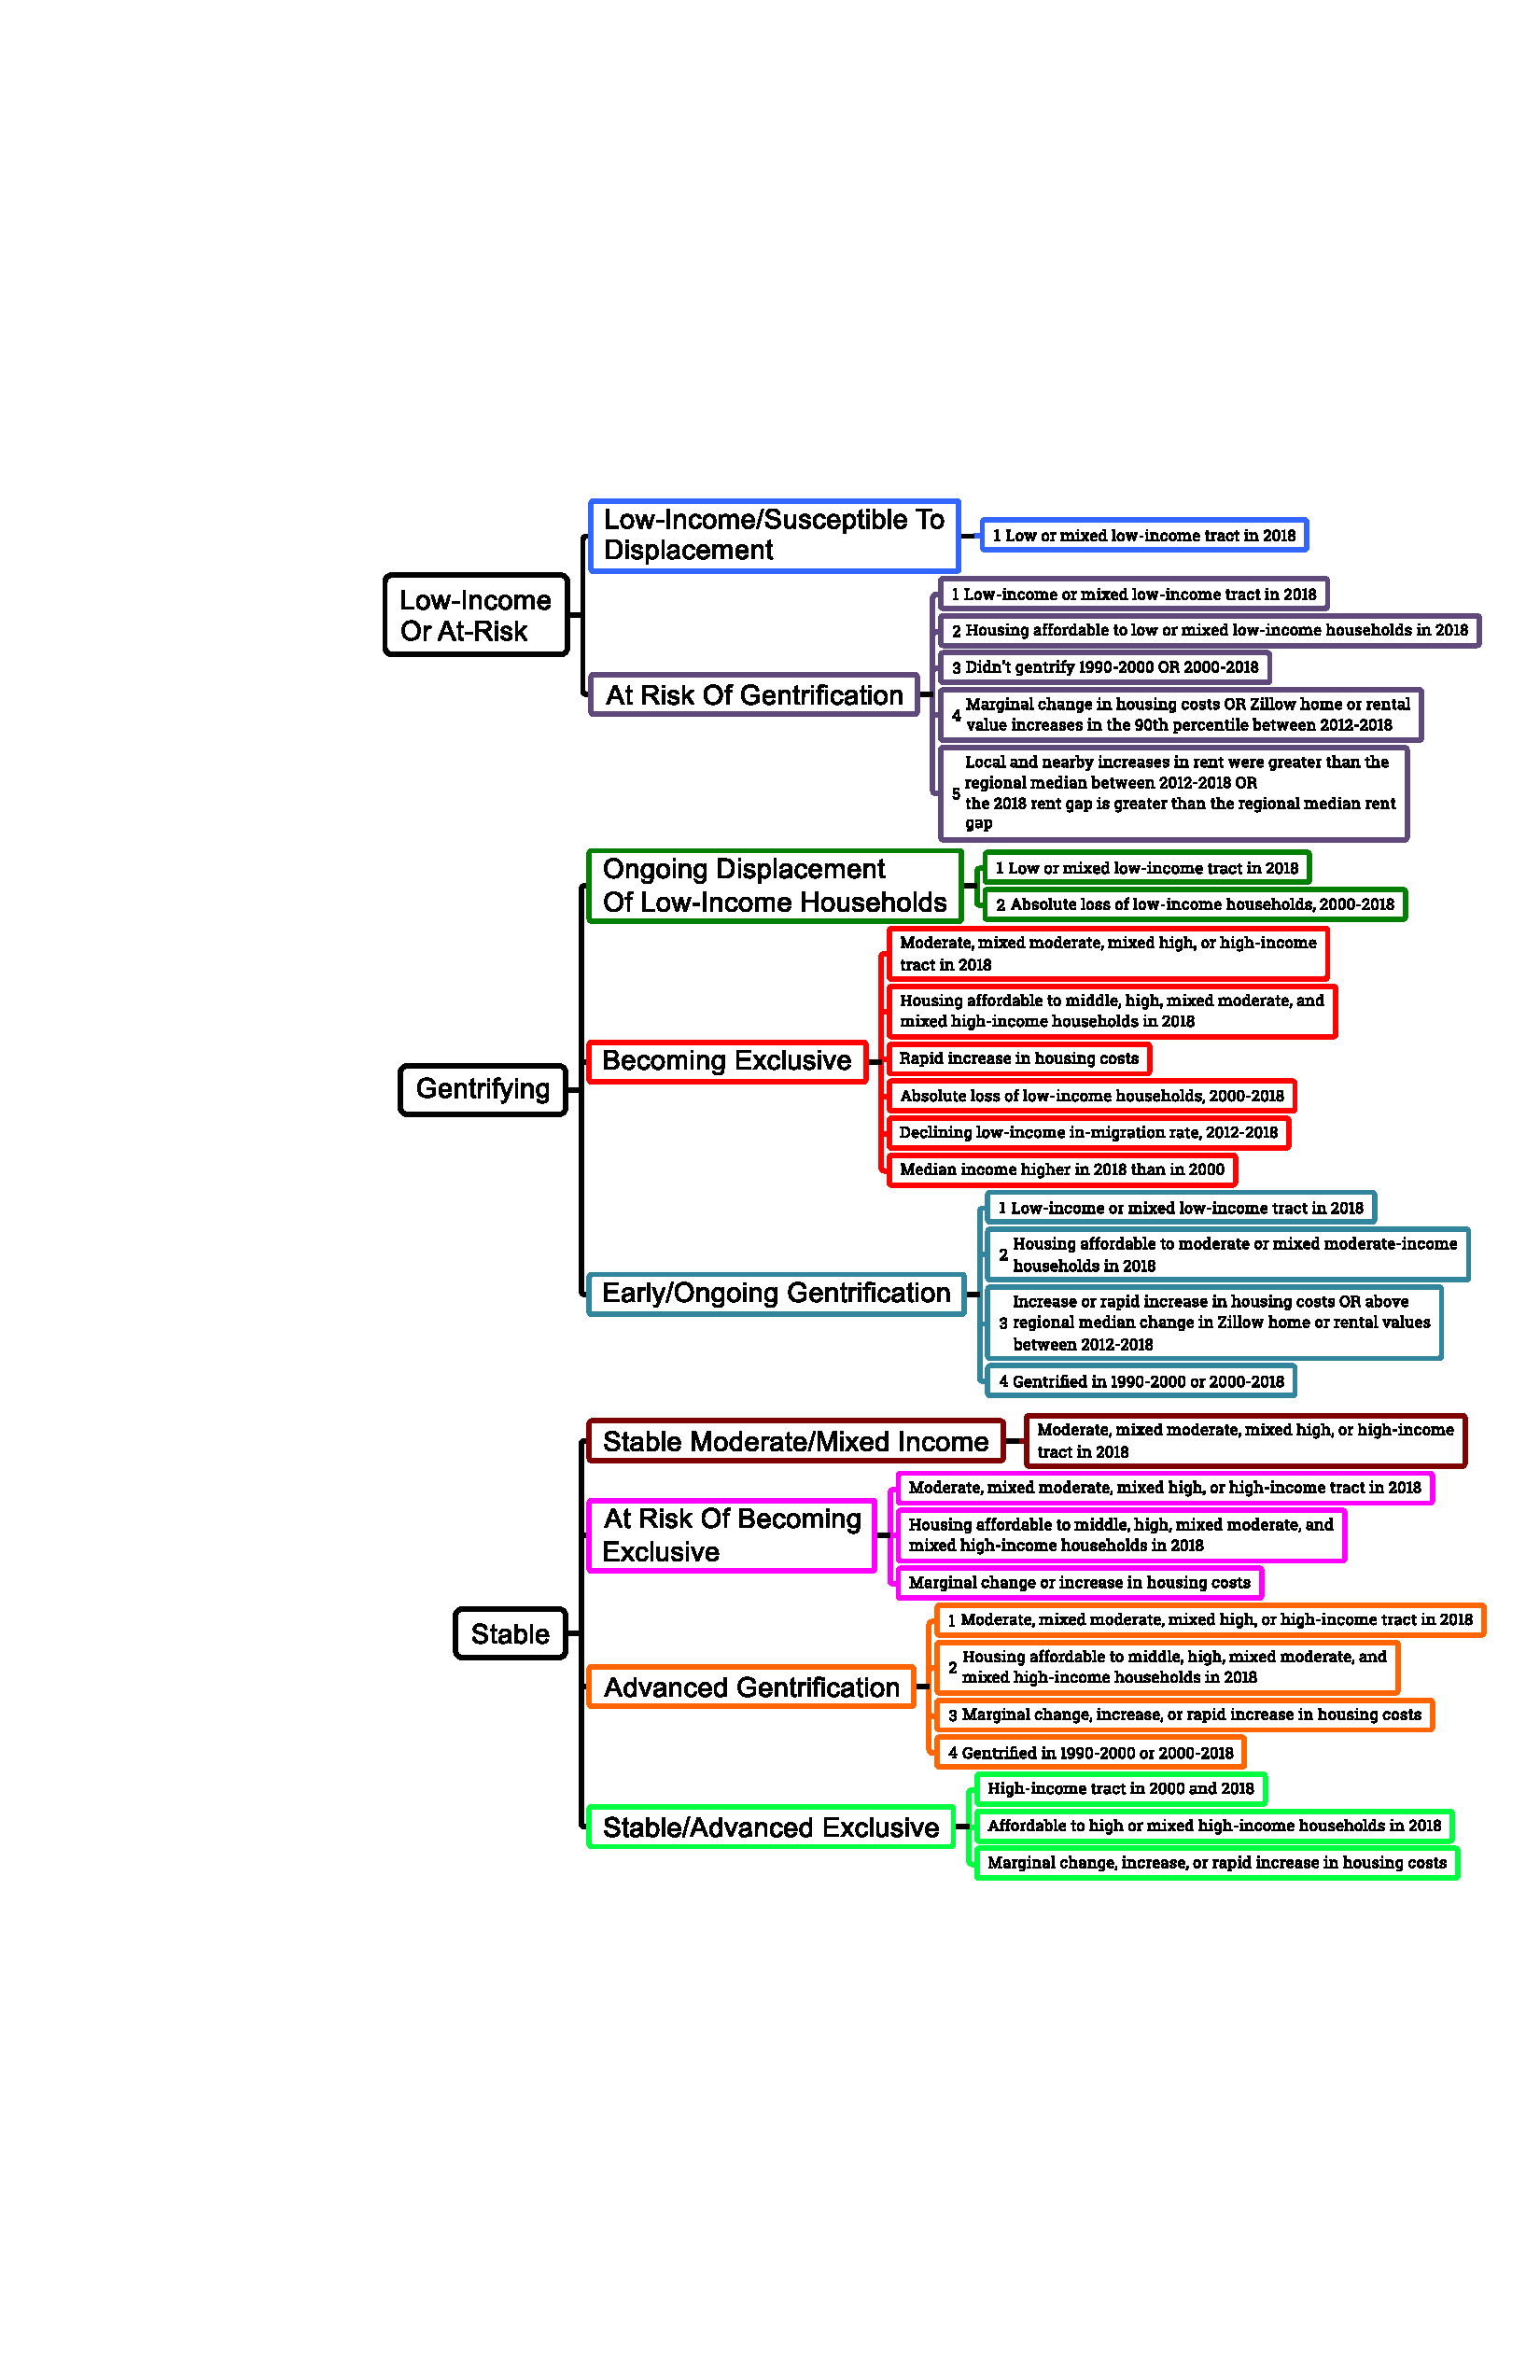
\includegraphics[width=\linewidth]{images/modified_typologies}
  \captionsetup{justification=centering, singlelinecheck=false, margin=2cm}
  \caption[Modified UDP Displacement Typologies]{Modified Urban Displacement Project (UDP) Typologies.}
  \label{fig:modified_typologies}
\end{figure}

\section{Operationalization}\

The dependent variable for this project is the number of fatal police uses of force. For purposes of this project, \acrfull{luof} will include those incidents in which the \textit{highest force used} is coded as tasered, gunshot, stabbed, asphyxiated\slash{}restrained, beaten\slash{}bludgeoned with an instrument, chemical agent\slash{}pepper spray, asphyxiation/restrained, or less than lethal force. The highest force used categories excluded are: vehicle, fell from a height, drowned, medical emergency, other, burned\slash{}smoke inhalation, drug overdose, and undetermined. Those categories included best reflect the direct use of force by an officer during an interaction, whereas the excluded \textit{highest force used} categories include incidents where no direct physical intervention was employed, and the officer merely happened to be present during a medical emergency or a drug overdose. The most frequently observed of the excluded categories, vehicle, could include incidents where officers never physically restrained the suspect, and the suspect had simply fled recklessly. Independent variables include: the race of the victim and the racial composition of the census tract, the median household income of the census tract, and the stage of gentrification or its absence within the tract.

\section{Hypotheses}

\noindent
\begin{tabular}{@{} l @{\hspace{18pt}} p{432pt} @{}}
$\textbf{H}_1$: &\acrshort{luof} rates should vary more substantially by income quintiles within each racial group than by racial groups within each income quintile. The lowest income quintiles should have the highest \acrshort{luof} rates.
\end{tabular}

\noindent
\begin{tabular}{@{} l @{\hspace{18pt}} p{432pt} @{}}
$\textbf{H}_2$: &Tracts experiencing gentrification or vulnerable to becoming gentrified should experience higher rates of \acrshort{luof} than higher-income tracts that have experienced no gentrification, regardless of the racial composition of the tract. That is, there should be more variation within each racial group by gentrification typology than there is within each gentrification typology by majority race.
\end{tabular}

\vspace{12pt}

To test these hypotheses, tracts were categorized as majority-black, majority-white, or majority-Hispanic/Latino. “Majority” shall mean greater than 50 percent of the tract is one of the three aforementioned racial groups. Other races and ethnicities will not be included in this typology, though they will be included in the denominators in calculating proportions to determine if any one group constitutes a majority. The race of the victim is specified in most of the entries in the data set of lethal uses of police force. Finally, all tracts will be binned into quintiles based on their median household income. Initial calculations will be done strictly using income quintiles. Per capita rates are calculated as follows:

\begin{equation}
{Rate}_q=\frac{{LUOF\_Count}_q}{{Population}_q}\times\frac{1}{6}\times10,000,000
\label{eq:quintile_rate}
\end{equation}

\noindent{}where \texttt{q} is the income quintile, \texttt{LUOF\_Count} is the number of \acrshort{luof}s that occurred in that income quintile, and \texttt{Population} is the total number of persons living in that particular income quintile. Per capita rates were annualized by dividing by six (the number of years in the study) and rescaled to a rate of “per 10 million.” Lethal use of force counts were then cross-tabulated for tract groups according to their respective income quintile and majority-race status: $\texttt{LUOF\_Count}_\texttt{mq}$, where \texttt{LUOF\_Count} is the total number of lethal uses of force that occurred in tracts with income quintile \texttt{q} and with a majority-race \texttt{m}, resulting in a table:

\begin{table}[H]
\centering
\begin{tabular}{cccc} %{matrix}
Income&Black&Latino&White\\
Q$_1$ &---&---&---\\
Q$_2$ &---&---&---\\
Q$_3$ &---&---&---\\
Q$_4$ &---&---&---\\
Q$_5$ &---&---&---\\
\end{tabular}
  \captionsetup{justification=centering, singlelinecheck=false, margin=2cm}
  \caption[LUOF Frequency: Majority-race and Income Quintile]{LUOF Frequency by Majority-race and Income Quintile.}
  \label{tab:luof_freq_majority_quintile}
\end{table}

Again, per capita rates were calculated by dividing \texttt{LUOF\_Count} by six (the number of years in the study), dividing by the number of persons of that particular race living in that particular income quintile, and multiplying by 10 million, to obtain the annualized rate per 10 million:

\begin{equation}
{Rate}_{qm}=\frac{{LUOF\_Count}_{qm}}{{Population}_{qm}}\times\frac{1}{6}\times10,000,000
\label{eq:quintile_majority_rate}
\end{equation}

The same scheme was employed to calculate the rates for the various gentrification typologies. First, rates were calculated for the Urban Displacement Project’s (\acrshort{udp}) gentrification typologies, \texttt{UDP}, without respect to the majority-race classification or the race of the victim. Then rates will be cross-tabulated for \texttt{UDP} by \texttt{Majority}, \texttt{UDP} by \texttt{Victim\_Race}), and \texttt{UDP} by \texttt{Majority} by \texttt{Victim\_Race}). With this, bar plots can be generated to assess how strongly each variable is related to the incidence of \acrshort{luof}s. Bringing in three dimensions to the analysis simultaneously can often illuminate a dynamic or interaction that otherwise goes unnoticed. For instance, there is often a question both in terms of how individuals are perceived based on ascription (race, gender, etc.), and other environmental factors, such as the racial composition of the neighborhood or forces of gentrification and how those might be related to a greater probability of being killed by law enforcement. Taking this three-way factor approach makes it possible to look at all these at the same time rather than in isolation.

Lastly, while I expect to find that class and gentrification indicators largely predict a greater incidence of \acrshort{luof}s than race alone, discrimination is also a causal force that does to some extent operate independently of economic factors, so I would expect some racial disparity to remain even after controlling for income and gentrification. In the final analysis, considering both how discrimination plays a role and how class and political economy have causal effects will enhance our understanding of the phenomenon.

\part{LITERATURE REVIEW}\

The literature in political science on the question of police killing has focused on the question of racial disparity. For example, a controversial article published in The National Academy of Sciences (PNAS) in 2019 asserted that the authors found “no evidence of anti-Black or anti-Hispanic disparities across shootings, and White officers are not more likely to shoot minority civilians than non-White officers” \parencite[15877]{johnsonOfficerCharacteristicsRacial2019}. This caused quite an uproar across the social sciences. Political Scientists Dean Knox and Jonathan Mummolo were among some of the more vocal critics. They voiced an issue with the methods that the authors used and published a short response \parencite{knoxMakingInferencesRacial2020}. Another lengthier article published later by \textcite{knoxAdministrativeRecordsMask2020} elucidated the authors’ claims more comprehensively. Their primary claim is that racial disparities exist and could even be underestimated because of the lack of data concerning when officers choose not to investigate; that is, there is no way of tracking how many whites they choose not to stop.

However, Adolph Reed Jr (\citeyear{reedHowRacialDisparity2016}), professor emeritus of political science at the University of Pennsylvania, has emphasized the limitations of race politics in combating the issue. He critiqued the antiracist orientation to the question both on normative grounds, in that, “antiracist politics is in fact the left wing of neoliberalism in that its sole metric of social justice is opposition to disparity in the distribution of goods and bads in the society, an ideal that naturalizes the outcomes of capitalist market forces so long as they are equitable along racial (and other identitarian) lines,” and on empirical grounds: “when we step away from focus on racial disproportions, the glaring fact is that whites are roughly half or nearly half of all those killed annually by police. And the demand that we focus on the racial disparity is simultaneously a demand that we disattend from other possibly causal disparities” (\cite{reedHowRacialDisparity2016}).

For example, \textcite{reedHowRacialDisparity2016} found that no blacks were killed in some of the states that experienced the highest rates of police killings. Moreover, \textcite{reedHowRacialDisparity2016} references that \parencite{jilani95PoliceKillings2015} found that 95 percent of police killings occurred in neighborhoods with median incomes under \$100,000, and “the average neighborhood family income where a killing occurred was \$57,764.” He contends that policing as an institution manages the social consequences produced by “the regime of market-driven public policy and increasing direction of the state’s functions at every level toward supporting accelerating regressive transfer.” Reed concludes by noting that “the focus on racial disparity accepts the premise of neoliberal social justice that the problem of inequality is not its magnitude or intensity in general but whether or not it is distributed in a racially equitable way.” Along with Reed, Political Scientist Cedric Johnson has studied the incorporation of the black political class into American politics post-1965 Voting Rights Act and the ways in which class cleavages among blacks are at least as important as interracial dynamics. This is important in at least two ways: one is that positing the issue of police killings and broader miscarriages of the criminal justice system strictly as racial in nature tends to paper over the role of black politicos in bringing about those outcomes in their adopting of austerity measures and advancing real estate developer interests and the concomitant repressive policing practices (\citeauthor{johnsonAfterwordBaltimorePolicing2016} \citeyear[305]{johnsonAfterwordBaltimorePolicing2016}; \citeyear[179]{johnsonTrumpismPolicingProblem2019}). The other is that the rhetoric of Black Lives Matter and cognate notions like the \textit{New Jim Crow}, popularized by Michelle Alexander’s (\citeyear{alexanderNewJimCrow2010}) book by the same name, “posit[] universal black injury where, in fact, police brutality and the carceral state are experienced more broadly across the working class” \parencite*[317]{johnsonAfterwordBaltimorePolicing2016}.

\section{Historical Perspective}\

Political Scientist Cedric Johnson looks at the question by examining policing historically, tracing back the emergence of today’s policing not to slave patrols or the perpetuation of the Jim Crow order but to the “discrete social contradictions of ‘postindustrial capitalism’” \parencite*[171]{johnsonTrumpismPolicingProblem2019}. \citeauthor{johnsonTrumpismPolicingProblem2019} argues that policing, since its modern inception, has always been about “disciplining the poor and protecting emergent property regimes” \parencite*[172]{johnsonTrumpismPolicingProblem2019}. In particular, he argues that the postwar transformation of US cities into middle-class suburbs with a high standard of living and the broader transformation of society into one of consumers produced a fundamental contradiction in that insofar as it produced middle-class suburbs, it also produced an “industrial reserve of unemployed, mostly black and brown urban dwellers” \parencite*[171]{johnsonTrumpismPolicingProblem2019}. In this context,

\begin{quote}
policing took a dual form: an emulatory strategy of promoting civic virtues of deference and middle-class aspiration, and a punitive strategy of defending the propertied and virtuous middle class from the outsiders, those segregated in inner-city ghettos and struggling to survive. \parencite[176]{johnsonTrumpismPolicingProblem2019}
\end{quote}

The Reagan and Bush years saw an intensification of what Johnson described as “class war at the urban level.” This included a rollback of the welfare state and a concomitant expansion of the carceral state and its more aggressive policing practices in urban minority communities \parencites[177]{johnsonTrumpismPolicingProblem2019}{johnsonBlackLivesMatter2023}. With the rise of gentrification, the urban landscape shifted once again with the physical distance created by the suburban, post-war transformation disappearing as the middle class began to reenter cities. Real estate speculation brought “urban pioneers, house flippers, large real estate developers, and tourists” into direct confrontation with the “old ethnic neighborhoods, the unemployed, the itinerant poor, sexual minorities, and countercultural spaces” \parencite[177]{johnsonTrumpismPolicingProblem2019}. According to Johnson, these class contradictions are managed through “manifold technologies of policing, surveillance, and social accreditation that permit ease of movement across urban space for those of means, while regulating and constricting the poor” \parencite*[178]{johnsonTrumpismPolicingProblem2019}. Johnson further elaborates that this new urban landscape is,

\begin{quote}
defined by helipads and Uber Black, artisanal grocers, boutique fitness clubs, private roads, dog parks, and relentless condo tower construction for the investor class and renascent bon vivant, and “bum-proof” benches, ankle monitors, stress policing, the demolition of public housing, water shutoffs, ubiquitous closed-circuit cameras, and check-cashing centers for the working-class enclaves. \parencite[178]{johnsonTrumpismPolicingProblem2019}.
\end{quote}

Thus, modern policing has a racist dynamic, but it is not about bias or other psychologistic notions like prejudice but is rooted in maintaining the capitalist social order. 

\section{Quantitative Analysis}\

Quantitative work backs Johnson’s claims. \citeauthor{feldmanPoliceRelatedDeathsNeighborhood2019}'s \parencite*{feldmanPoliceRelatedDeathsNeighborhood2019} study looked at the association between rates of police-related deaths and indices of neighborhood residential segregation using several measures that included income, race/ethnicity, or both. They used the American Community Survey’s 5-year estimates to obtain census tract data, and the \acrfull{ice} to operationalize segregation. \acrshort{ice} allows researchers to “simultaneously measure[] the relative concentrations of privileged and deprived residents in an area” \parencite[459]{feldmanPoliceRelatedDeathsNeighborhood2019}. While \acrshort{ice} had previously been used to operationalize privileged and deprived status in terms of income alone, it has since been broadened to include other considerations, such as racial/ethnic privilege and deprivation. In this case, Feldman et al. used 5 common \acrshort{ice} measures, defining privilege and deprivation in terms of: (1) high- versus low-income neighborhoods, (2) non-Hispanic white versus non-Hispanic black persons, (3) non-Hispanic white versus \acrfull{poc}, (4) high-income non-Hispanic White versus low-income Black households, and (5) high-income non-Hispanic White versus low-income \acrshort{poc} households. Each \acrshort{ice} score ranged from -1 to 1, with -1 indicating 100 percent of the population belonging to the most deprived group and 1 signifying that 100 percent of the population belonged to the most privileged group \parencite[459]{feldmanPoliceRelatedDeathsNeighborhood2019}. In addition to the census tract measures, they included characteristics of the individuals killed in the tracts in their analyses.

\citeauthor{feldmanPoliceRelatedDeathsNeighborhood2019} found that, for the years in the study (2015-16), “census tract concentrations of economic privilege were associated with lower rates of police-related deaths,” and “greater concentrations of deprivation were associated with higher rates” \parencite*[461]{feldmanPoliceRelatedDeathsNeighborhood2019}. At the same time, \acrshort{ice} measures for racialized economic polarization did not show a meaningful difference “compared with \acrshort{ice} measures of census tract income or census tract race/ethnicity alone (2019, 461). The most privileged quintile of census tracts experienced police-related killings at roughly half the rate of the second most privileged quintile, regardless of whether privilege was measured solely in terms of income, by income and race/ethnicity, or by poverty \parencite*[461]{feldmanPoliceRelatedDeathsNeighborhood2019}. Individual-level analysis in combination with the tract characteristics provided an additional layer. For example, when privilege and deprivation were defined solely by census tract racial/ethnic concentration, only non-Hispanic whites experienced a lower risk of being killed by law enforcement in tracts with the highest concentration of white residents, while non-Hispanic blacks experienced a higher risk of being killed by law enforcement in census tracts with higher concentrations of non-Hispanic whites \parencite*[461]{feldmanPoliceRelatedDeathsNeighborhood2019}.

In another study, \textcite{feldmanPoliceKillingsUS2020} took a slightly different methodological approach. First, he separated census tracts by poverty quintiles. He obtained police killings data and again located the census tracts where those incidents occurred. Using that data, he was able to calculate the annualized per capita police killing rate of each poverty quintile. He found that,

\begin{quote}
within all three racial/ethnic groups, rates of police killings were higher with increasing census tract poverty…. The relationship between poverty quintile and police killings was strongest for whites, for whom the rate was nearly 4-fold higher in the highest-poverty quintile…. For the black population, the police killing rate was 1.8-fold higher in the highest-poverty quintile relative to the lowest-poverty quintile…. The relationship was weakest for Latinos. \parencite{feldmanPoliceKillingsUS2020}
\end{quote}

\noindent{}That is, poverty was associated with higher rates of police killings for all racial/ethnic groups, with the association the strongest for whites and weakest for Latinos and with blacks somewhere in between in terms of strength of the association.

One question that remained was that since blacks and Latinos have higher poverty rates, how much of the difference in rates of police killings between races and ethnicities could be explained statistically as a function of differences in poverty rates in general? To answer that, he constructed a counterfactual scenario in which the poverty rates for blacks and Latinos were adjusted to be on the same scale as whites, scaling the per capita rates of police killings accordingly. He found that under the counterfactual poverty scenario in which black poverty was equal to white poverty, police killings would diminish from the observed rate (7.9 per million) to 6.6 per million, “a 28 percent reduction in the white-black gap in police killing rates on the additive scale” \parencite{feldmanPoliceKillingsUS2020}. For Latinos, the rate diminished from the observed rate of 3.5 per million to 3.1 per million, which was lower than the observed rate for whites. Because of this, Feldman contends, “the poverty distribution is sufficient to explain the Latino-white gap in police killings” \parencite{feldmanPoliceKillingsUS2020}.

\section{An Analysis of Space}\

Lo\"ic \textcite{wacquantClassRaceHyperincarceration2010} locates the origins of the related phenomenon of incarceration in the diminution of the \textit{social state} and the corresponding rolling out of the penal state. This political transformation has altered the “modalities of action of public authority when it comes to managing the deprived and stigmatized populations stuck at the bottom of the class, ethnic, and urban hierarchy” \parencite[74]{wacquantClassRaceHyperincarceration2010}. And this phenomenon is not easily explained by trends in poverty rates or crime. Rather, it is “fueled by a politics of resentment,” where stigmatized populations are portrayed as undeserving public-aid recipients and street criminals, popularly condensed as the “black underclass” \parencite[74]{wacquantClassRaceHyperincarceration2010}.

\textcite{wacquantClassRaceHyperincarceration2010} brings in an analysis of space that others have neglected. He argues that the intensification of police activities has targeted people by class, race, and space. This triple selectivity has led not to what some have called “mass incarceration,” but to \emph{hyper-incarceration}, affecting the lowest end of the African-American working class. This punitive turn occurred at the dawn of the post-Fordist era, as the US turned to a postindustrial service economy with a greater share of insecure and precarious labor.

The other element in the expansion of the penal system is its horizontal dimension. This includes the population typically not counted as part of the incarcerated—parolees and probationers, or those otherwise restricted in their movement or activities by the criminal justice system. \citeauthor{wacquantClassRaceHyperincarceration2010} contends that this ought to be considered “an extension of the custodial system, rather than an alternative to it” (\citeyear[76]{wacquantClassRaceHyperincarceration2010}; italics in original). This coincided with greater surveillance technologies, such as the expansion of offender databases to include not only mugshots and fingerprints but also DNA prints and the proliferation of categories of convicts, such as sex offenders, which sought “to expurgate specific categories…from the social body” \parencite[76]{wacquantClassRaceHyperincarceration2010}.

These are the characteristics of what \citeauthor{wacquantClassRaceHyperincarceration2010} has termed \emph{hyperincarceration}—the concentration of this policing regime in the black, urban ghetto; its principal targets, “lower-class African American men” \parencite*[78]{wacquantClassRaceHyperincarceration2010}. To understand the phenomenon, He employs the term triple selectivity—the “filter” that sorts those who are subject to inclusion in the expansion of the carceral state, and those who are largely exempt. The first filter is class. \citeauthor{wacquantClassRaceHyperincarceration2010} notes that, “The welcome focus on race, crime, and punishment that has dominated discussions of the prison boom has obliterated the fact that inmates are first and foremost poor people… This clientele is drawn overwhelmingly from the most precarious fraction of the urban working class” (\citeyear[78--79]{wacquantClassRaceHyperincarceration2010}; italics in original). The second filter is race. \citeauthor{wacquantClassRaceHyperincarceration2010} notes that, while the prison population used to be 70 percent white and 30 percent “other” in the 1960s-70s, it “flip-flopped” to “70 percent African American and Latino versus 30 percent white by the century’s end” \parencite*[79--80]{wacquantClassRaceHyperincarceration2010}. But the racial dimension has been more “class disproportionate” inside each racial or ethnic category than it has been racially disproportionate between them \parencite*[80]{wacquantClassRaceHyperincarceration2010}. Citing sociologist Bruce Western, he notes that “the cumulative risk of imprisonment for African American males without a high school diploma tripled between 1979 and 1999,” to 59 percent, but during the same period, the risk for “African American men with some college education decreased from 6 percent to 5 percent” \parencite*[79]{wacquantClassRaceHyperincarceration2010}.


%travisGrowthIncarcerationUnited2014

\part{CONCLUSION}\

{\color{red}[Conclusion goes here]}

\clearpage
\part{APPENDIX}

\begin{figure}%[H]
  \centering % width=\linewidth, height=\textheight
  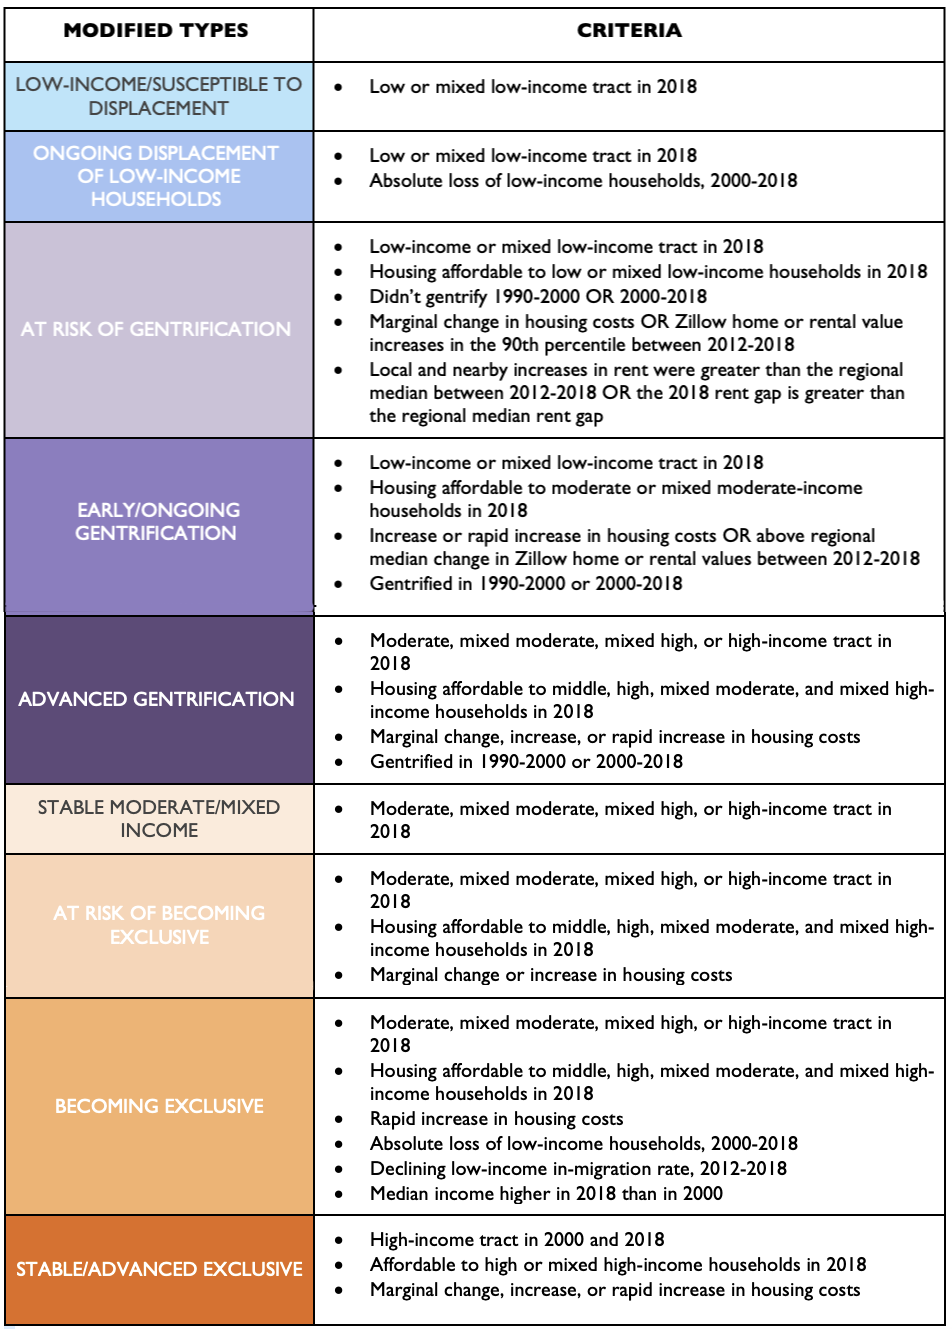
\includegraphics[height=0.95\textheight]{images/typology_sheet_2018}
  \captionsetup{justification=centering, singlelinecheck=false, margin=2cm}
  \caption[UDP Displacement Typologies]{Original Urban Displacement Project (UDP) Typologies.}
  \label{fig:original_udp}
\end{figure}

\clearpage
\sloppy


\titleformat{\section}{\fontsize{12}{14}\bfseries\centering}{\thesection}{0.5em}{}
% Line spacing
\setstretch{1.25}
\printbibliography[heading=bibintoc]

%\clearpage

%\paperwidth=\pdfpageheight
%\paperheight=\pdfpagewidth
%\pdfpageheight=\paperheight
%\pdfpagewidth=\paperwidth
%\headwidth=\textheight
%\begingroup 
%\vsize=\textwidth
%\hsize=\textheight

%\newpage
%\paperwidth=\pdfpageheight
%\paperheight=\pdfpagewidth
%\pdfpageheight=\paperheight
%\pdfpagewidth=\paperwidth
%\headwidth=\textwidth

\end{document}
